% Generated by code/needham.py -- do not edit by hand.
\definecolor{qocA}{rgb}{0.00,0.45,0.70}
\definecolor{qocB}{rgb}{0.90,0.60,0.00}
\definecolor{qocC}{rgb}{0.00,0.62,0.45}
\definecolor{qocD}{rgb}{0.80,0.40,0.00}
\definecolor{qocE}{rgb}{0.80,0.60,0.70}
\definecolor{qocF}{rgb}{0.35,0.70,0.90}
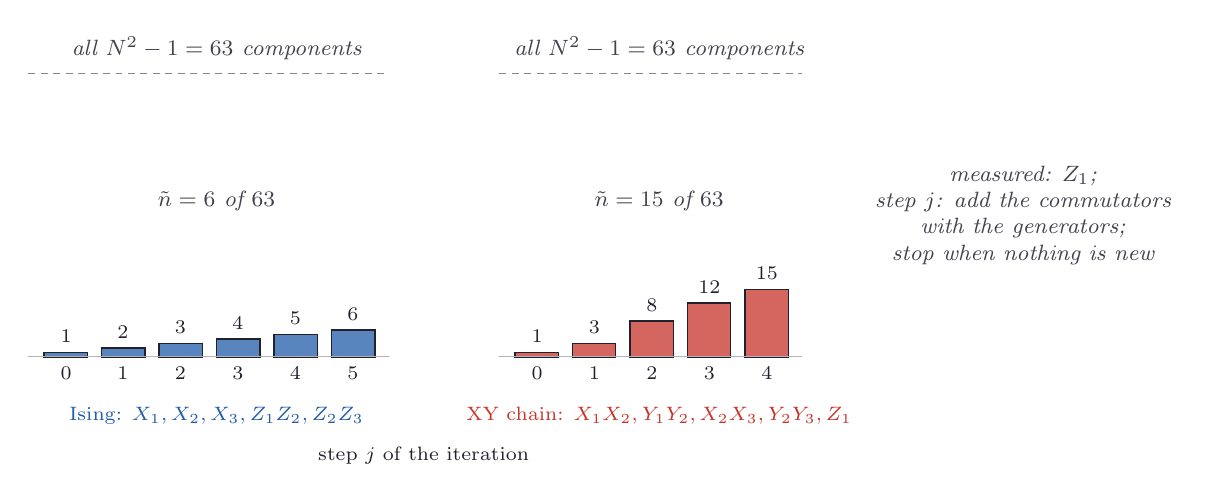
\begin{tikzpicture}[ink/.style={line width=0.9pt, ndInk}, faint/.style={line width=0.4pt, ndInk!35}, dashedink/.style={line width=0.5pt, ndInk!55, dash pattern=on 2.5pt off 2pt}, vec/.style={->, >=stealth, line width=1.2pt}, note/.style={font=\footnotesize\itshape, text=ndInk!85, align=center}, pointer/.style={->, >=stealth, line width=0.4pt, ndInk!60, shorten >=2pt, shorten <=1pt}, dot/.style={circle, fill=ndInk, inner sep=0pt, minimum size=3.4pt}, wash/.style={fill=ndSky, fill opacity=0.55}, every node/.style={text=ndInk}]
\definecolor{ndInk}{rgb}{0.13,0.13,0.18}
\definecolor{ndPaper}{rgb}{0.99,0.96,0.88}
\definecolor{ndSky}{rgb}{0.84,0.91,0.98}
\definecolor{ndRose}{rgb}{0.98,0.86,0.84}
\definecolor{ndBlue}{rgb}{0.13,0.36,0.66}
\definecolor{ndRed}{rgb}{0.78,0.20,0.16}
\definecolor{ndGold}{rgb}{0.88,0.62,0.10}
\definecolor{ndGreen}{rgb}{0.18,0.52,0.30}
\fill[ndBlue, fill opacity=0.75] (0.00,0) rectangle (0.55,0.057);
\draw[ink, line width=0.5pt] (0.00,0) rectangle (0.55,0.057);
\node[font=\scriptsize, above] at (0.28,0.057) {1};
\node[font=\scriptsize, below] at (0.28,0) {0};
\fill[ndBlue, fill opacity=0.75] (0.73,0) rectangle (1.28,0.114);
\draw[ink, line width=0.5pt] (0.73,0) rectangle (1.28,0.114);
\node[font=\scriptsize, above] at (1.00,0.114) {2};
\node[font=\scriptsize, below] at (1.00,0) {1};
\fill[ndBlue, fill opacity=0.75] (1.46,0) rectangle (2.01,0.171);
\draw[ink, line width=0.5pt] (1.46,0) rectangle (2.01,0.171);
\node[font=\scriptsize, above] at (1.73,0.171) {3};
\node[font=\scriptsize, below] at (1.73,0) {2};
\fill[ndBlue, fill opacity=0.75] (2.19,0) rectangle (2.74,0.229);
\draw[ink, line width=0.5pt] (2.19,0) rectangle (2.74,0.229);
\node[font=\scriptsize, above] at (2.46,0.229) {4};
\node[font=\scriptsize, below] at (2.46,0) {3};
\fill[ndBlue, fill opacity=0.75] (2.92,0) rectangle (3.47,0.286);
\draw[ink, line width=0.5pt] (2.92,0) rectangle (3.47,0.286);
\node[font=\scriptsize, above] at (3.19,0.286) {5};
\node[font=\scriptsize, below] at (3.19,0) {4};
\fill[ndBlue, fill opacity=0.75] (3.65,0) rectangle (4.20,0.343);
\draw[ink, line width=0.5pt] (3.65,0) rectangle (4.20,0.343);
\node[font=\scriptsize, above] at (3.92,0.343) {6};
\node[font=\scriptsize, below] at (3.92,0) {5};
\draw[faint] (-0.20,0) -- (4.38,0);
\draw[dashedink] (-0.20,3.600) -- (4.38,3.600);
\node[note, anchor=south] at (2.19,3.650) {all $N^2-1=63$ components};
\node[font=\scriptsize, text=ndBlue] at (2.19,-0.75) {Ising: $X_1,X_2,X_3,Z_1Z_2,Z_2Z_3$};
\node[note] at (2.19,1.980) {$\tilde n=6$ of $63$};
\fill[ndRed, fill opacity=0.75] (5.98,0) rectangle (6.53,0.057);
\draw[ink, line width=0.5pt] (5.98,0) rectangle (6.53,0.057);
\node[font=\scriptsize, above] at (6.26,0.057) {1};
\node[font=\scriptsize, below] at (6.26,0) {0};
\fill[ndRed, fill opacity=0.75] (6.71,0) rectangle (7.26,0.171);
\draw[ink, line width=0.5pt] (6.71,0) rectangle (7.26,0.171);
\node[font=\scriptsize, above] at (6.99,0.171) {3};
\node[font=\scriptsize, below] at (6.99,0) {1};
\fill[ndRed, fill opacity=0.75] (7.44,0) rectangle (7.99,0.457);
\draw[ink, line width=0.5pt] (7.44,0) rectangle (7.99,0.457);
\node[font=\scriptsize, above] at (7.72,0.457) {8};
\node[font=\scriptsize, below] at (7.72,0) {2};
\fill[ndRed, fill opacity=0.75] (8.17,0) rectangle (8.72,0.686);
\draw[ink, line width=0.5pt] (8.17,0) rectangle (8.72,0.686);
\node[font=\scriptsize, above] at (8.45,0.686) {12};
\node[font=\scriptsize, below] at (8.45,0) {3};
\fill[ndRed, fill opacity=0.75] (8.90,0) rectangle (9.45,0.857);
\draw[ink, line width=0.5pt] (8.90,0) rectangle (9.45,0.857);
\node[font=\scriptsize, above] at (9.18,0.857) {15};
\node[font=\scriptsize, below] at (9.18,0) {4};
\draw[faint] (5.78,0) -- (9.63,0);
\draw[dashedink] (5.78,3.600) -- (9.63,3.600);
\node[note, anchor=south] at (7.81,3.650) {all $N^2-1=63$ components};
\node[font=\scriptsize, text=ndRed] at (7.81,-0.75) {XY chain: $X_1X_2,Y_1Y_2,X_2X_3,Y_2Y_3,Z_1$};
\node[note] at (7.81,1.980) {$\tilde n=15$ of $63$};
\node[note, anchor=west] at (10.43,1.8) {measured: $Z_1$;\\ step $j$: add the commutators\\ with the generators;\\ stop when nothing is new};
\node[font=\scriptsize] at (4.82,-1.25) {step $j$ of the iteration};
\end{tikzpicture}
